\section{Stovepipe Enterprise}

\subsection{Form \& Causes}

Stovepipe Enterprise, also know as Island of Automation \cite{c2com} is a situation when multiple system within enterprise are designed independently at every level \cite{Crisis}. Those systems has potential to share data, functionality or whole subsystems but they don't.

Stovepipe metaphor isn't accidental. Stovepipe is the pipe which conducts smoke from a coal or wood-burning stove to it's chimney. There are two problems with such pipes and two similar problems will occur in case of stovepipe enterprise anti-pattern. The first problem is that burning wood produces corrosive substances that erode metal, so pipe must be constantly maintained and repaired in order to avoid leakage. Second problem is fact that stovepipes are never connected with each other to create one system. If one would have a two coals he would have two separate stovepipes to maintain.

This analogy perfectly fits into stovepipe enterprise anti-pattern where we have separated systems which has to be maintained separately because of they layer separation. This and other problems will be discussed in the next chapter.

\begin{figure}[!h]
    \centering
    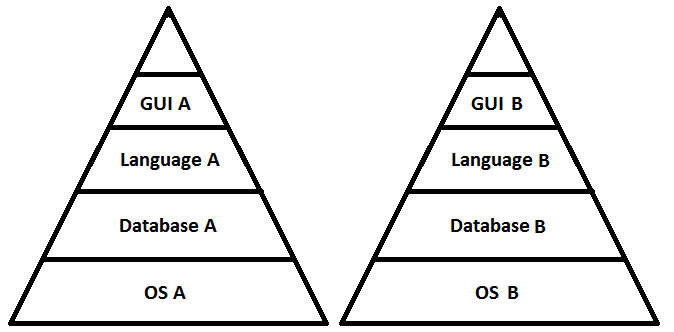
\includegraphics[scale=0.7]{Images/Systems.png}
    \caption[Stovepipe Enterprise Systems]{Stovepipe Enterprise Systems - example visualization}
    \label{fig:Systems}
\end{figure}

Causes of such situations are in general lac of standards, lac of communication and laziness. When a company have global system standards, technology strategy and system profiles then even without teems and enterprise institutions communication such anti-pattern could be avoided. Lack of communication, lack of knowledge about technology standards being used in company and absence of horizontal interfaces in system integration solutions are the main causes of the stovepipe enterprise anti-pattern \cite{SurvivalGuide}.
It can also came from rapid expansion of the company and systems - from few small applications to big enterprise systems \cite{Dragon}.

\subsection{Symptoms \& Consequences}

The main symptoms and consequences of the stovepipe enterprise anti-pattern are \cite{SurvivalGuide}:
\begin{itemize}
	\item Lack of software reuse between enterprise systems
	\item Lack of interoperability between enterprise systems
	\item Brittle systems
	\item Monolithic systems
	\item Undocumented architectures
	\item Inability to extend systems
	\item Excessive maintenance costs
	\item Employee turnover may causes project discontinuity and maintenance problems
\end{itemize}
Many of those consequences can be notices at the early stages of system creation. If some subsystem can be maintained only by one employ this is probably separate "island" of the system. If system architecture is known only to system team and there is no enterprise standard then undocumented architecture problem will occur. Also no one else outside the team would be able to quickly join to the team or connect two different systems.


\subsection{Example - authorization system}

As an example of the stovepipe enterprise anti-pattern will be considered a e-mail system and calendar system within one company.

Both systems besides they unique data had to store information about they users and passwords. In enterprise where are no standards on database layer defined we can expect that those systems can use different technologies, naming conventions and will probably not share the information. 
\hyperref[fig:DatabaseExample]{Figure \ref{fig:DatabaseExample}} shows tables for those two systems. In case where those systems uses different databases technologies the gap between database layer is even higher.

\begin{figure}[htp]
\subcaptionbox{E-mail system - example tables in MySQL database\label{fig:EmailSystem}}{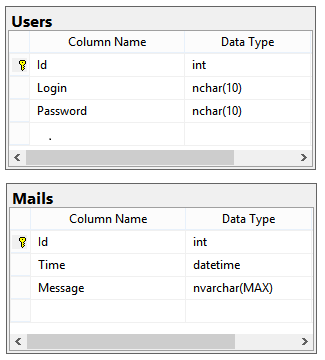
\includegraphics[width=.48\linewidth]{Images/semail.png}}\hfill%
\subcaptionbox{Calendar system - example tables in MSSSL database\label{fig:CalendarSystem}}{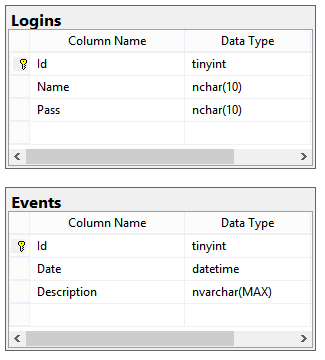
\includegraphics[width=.48\linewidth]{Images/secalendar.png}}%
\caption[Stovepipe Enterprise Systems database example]{Stovepipe Enterprise Systems database example - different tables in different databases technologies}
\label{fig:DatabaseExample}
\end{figure}

Not only the the separation of tables is the symptom of the stovepipe enterprise anti-pattern but also the different naming conventions and \emph{Id} field data type.
Such systems require double work in case of changing any user data in any of those two systems. So it is inconvenient both in development and in administration.

\newpage
\subsection[Solution]{Solution*}

\footnote{Due to lack of other source the whole chapter is based on \cite{SurvivalGuide}}
Coordination of technologies at each level is necessary to both avoid and solve stovepipe enterprise problem. Providing any enterprise design pattern will help future refactorization. Defining standards at each level is the first step and it should be done in order from the lowest level (high-level architecture) to the highest (API specifications, extensions etc).

Topic is new but the problem is old, so many large enterprises developed conventions for the definitions of object-oriented architectures that can be applied to many organizations. The key is to define detailed interoperability \footnote{Property of a product or system, whose interfaces are completely understood, to work with other products or systems, present or future, without any restricted access or implementation. \cite{Interoperability}} conventions across systems of large-scale architectures. And at the same time address technology strategy and requirements. Experience has shown that four requirements models and four specification models has to be defined in order to properly scope interoperability between layer.

\begin{figure}[!h]
    \centering
    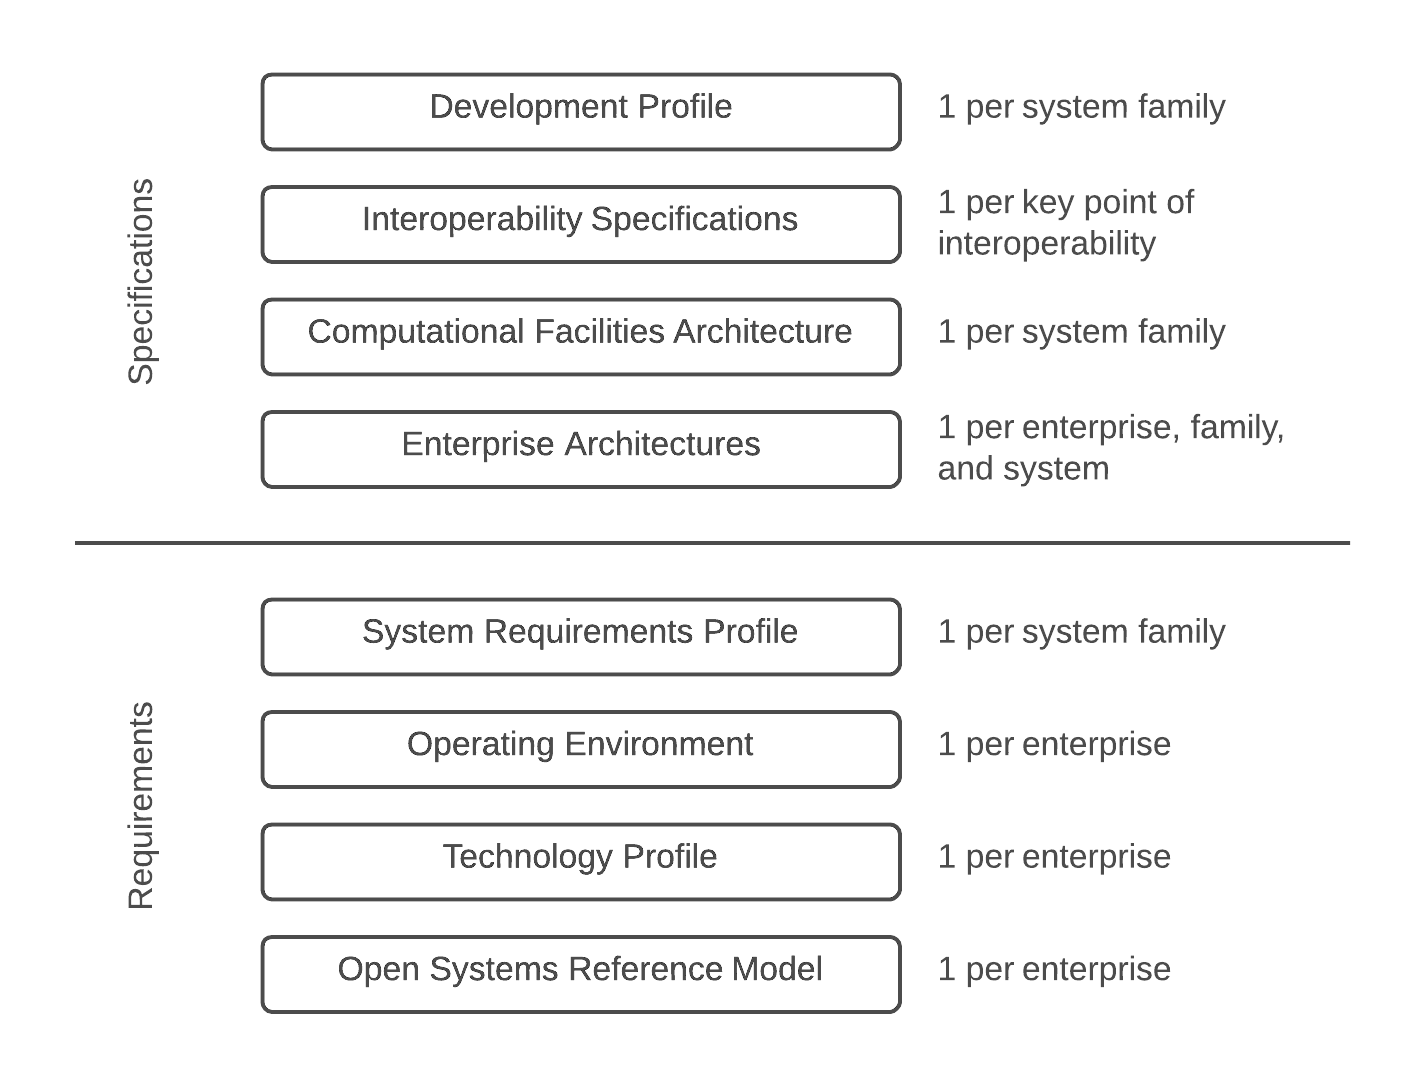
\includegraphics[scale=0.3]{Images/enterprisesolution.png}
    \caption[Scoping of interoperability]{Scoping of interoperability \cite{SurvivalGuide}}
    \label{fig:ScopingOfInteroperability}
\end{figure}
Detailed description of each layer will not be discussed.


\newpage
Based on that, the solution for the example database layer show on \hyperref[fig:DatabaseExample]{figure \ref{fig:DatabaseExample}} can be provided.
The first step will be to define one database technology, then the naming conventions and types standards. After that one table for all user for both systems can be defined as it is shown on \hyperref[fig:DatabaseExample]{figure \ref{fig:DatabaseExampleSolution}}.

\begin{figure}[!h]
    \centering
    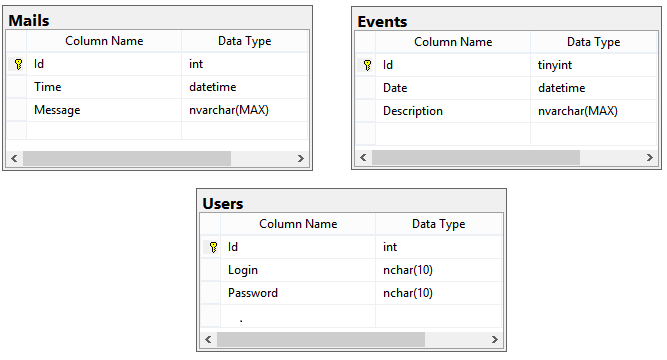
\includegraphics[width=\textwidth]{Images/sesolution.png}
    \caption[Example database layer - solution]{Example database layer - solution}
    \label{fig:DatabaseExampleSolution}
\end{figure}


\subsection{Exceptions}

Stovepipe Enterprise Anti-Pattern may occur in situations in which is acceptable.
In new systems and application is not, however when companies grow by takeover or merge occurrence of this anti-pattern can be expected. Vendor Lock-In Anti-Pattern can be an other exception \cite{SurvivalGuide}.
The situation when company grows by itself, when it starts from few small applications which are not well designed, there will be a point problems connected to stovepipe enterprise will show up \cite{Dragon}.

Besides Vendor Lock-In exception, all others are just temporary and should be refactored at the earliest state as possible.